\section{Desarrollo}

\subsection{Discusión Teórica}

Para efectuar los análisis del método de la matriz de Colley (CMM), se asume que ambos métodos de resolución: Eliminación Gaussiana (EG) y Factorización de Cholesky (CL) funcionan siempre. 

Es sabido que no todas las matrices admiten CL o el algoritmo EG y la implementación de ambos métodos en este Trabajo Práctico es fiel a los algoritmos presentados, con lo cual si la asunción previa no se cumple, las corridas que dan base a la experimentación serían indeterminadas (cuelgues de máquina o generación de resultados basura).

La justificación de que la asunción se cumple viene dada por el hecho de que la matriz de Colley desde su armado es simetrica definida positiva, como está explicado en el paper ''Colley's Bias Free College Football Ranking Method: The Colley Matrix Explained''  de W. Colley, sección 7.2

\begin{itemize}

\item SDP $\implies$ A inversible y todas las submatrices principales de A inversibles $\implies$ A tiene factorización LU

\item La factorización LU tal que L tenga 1s en su diagonal es unica

\end{itemize}

Si es única, debe ser la factorización obtenida por el algoritmo de elimincación Gaussiana por motivos constructivos, dado que esta tiene 1s en su diagonal.

\vspace{1em}

Propiedad: Sea \(A \in \mathbb{R}^{n \times n}\) Simétrica Definida Positiva \(\implies A\) No singular $land$ todas las submatrices principales de $A$ No singulares.

Demostración: Por absurdo:

\begin{itemize}

\item Supongamos que $A$ es Singular \(\implies \exists \tilde{x} \) tq \(A\tilde{x} = 0 \) con \(\tilde{x} \neq 0 \)

\begin{equation}
\tilde{x}^{T}\underbrace{A\tilde{x}}_{0} = 0 \text{\hspace{3em} Abs! porque $A$ es S.D.P \hspace{1em}} (x^{T}Ax > 0 \hspace{1em}\forall x \neq 0)
\end{equation}


Luego $A$ es No Singular

\item Sea $A_{k}$ la submatriz principal $\mathbb{R}^{k\times k}$ de $A \in \mathbb{R}^{n \times n}$

Supongo que $A_{k}$ es singular (No inversible) $\implies \exists \bar{x_k}$ tq $A_k \bar{x_k} = 0$ con $\bar{x_k} \neq 0$

\[\text{Sea } \bar{x_{k}} \in \mathbb{R}^{k} \text{tq } A_{k} \bar{x_{k}} = 0  \land \bar{x_{k}} \neq 0 \]

\[ \text{Sea } \bar{x} = \begin{pmatrix} \bar{x_{k}} \\ 0 \\ \vdots \\ 0 \end{pmatrix} \in \mathbb{R}^{n} \]

\begin{equation}
 \bar{x}^{T} A \bar{x} = \begin{pmatrix} \bar{x_{k}} & 0 & \cdots & 0 \end{pmatrix}
  \begin{blockarray}{ccccc|cccc}
    \begin{block}{(ccccc|cccc@{\hspace*{5pt}})}
	\BAmulticolumn{5}{c|}{\multirow{5}{*}{$A_{k}$}}&\BAmulticolumn{4}{c}{\multirow{5}{*}{}}\\
    &&&&&&&\\
    &&&&&&&\\
    &&&&&&&\\
    &&&&&&&\\
    \cline{1-5}% don't use \hline
    \BAmulticolumn{5}{c}{\multirow{4}{*}{}}&\BAmulticolumn{4}{c}{\multirow{4}{*}{}}\\
    \BAmulticolumn{5}{c}{\multirow{4}{*}{}}&\BAmulticolumn{4}{c}{\multirow{4}{*}{}}\\
    \BAmulticolumn{5}{c}{\multirow{4}{*}{}}&\BAmulticolumn{4}{c}{\multirow{4}{*}{}}\\
    \BAmulticolumn{5}{c}{\multirow{4}{*}{}}&\BAmulticolumn{4}{c}{\multirow{4}{*}{}}\\
    \end{block}
  \end{blockarray}
  \begin{pmatrix} \bar{x_{k}} \\ 0 \\ \vdots \\ 0 \end{pmatrix} =
  \begin{pmatrix} \bar{x_{k}} & 0 & \cdots & 0 \end{pmatrix}   \  \underbrace{\begin{pmatrix} 0 \\ \vdots \\ 0 \\ * \\ \vdots \\ * \end{pmatrix}}_{A \bar{x}} = 0
\end{equation}
Los primeros $k$ elementos del vector $A \bar{x}$ son iguales a $0$ dado que haciendo el producto por bloques de $A$ con $\bar{x}$ por cada fila de $A$ las $n-k$ ultimas columnas se anulan al ser multiplicadas por los $n-k$ ultimos ceros de $\bar{x}$ y el primer bloque de dimension $k \times 1$ del vector resultado ( $ = A_k \bar{x_{k}} )$ es cero por hipótesis.

El producto $\bar{x}^{T} (A \bar{x} )$ es igual a cero dado que los primeros $k$ elementos de $\bar{x}^{T}$ son multiplicados por los primeros $k$ ceros del producto $A \bar{x}$ y los $n-k$ ceros de $\bar{x}^{T}$ anulan los $n-k$ ultimos elementos de $A \bar{x}$

\[\text{Abs! pues } A \text{es SDP y } \bar{x} = \begin{pmatrix} \bar{x_{k}} \\ 0 \\ \vdots \\ 0 \end{pmatrix} \neq 0\]

O sea toda $A \in \mathbb{R}^{n \times n}$ SDP tiene todas sus submatrices principales no singulares y $A$ es no singular \qed

\end{itemize}

Propiedad: Sea $A \in \mathbb{R}^{n \times n}$ $A$ inversible (no singular), si las submatrices principales de $A$ son no singulares $\implies$ $A = L U$

Demostración: (x inducción)

\begin{itemize}
	\item $n = 2$
	
	Las hipótesis son:
	\[ A = \begin{pmatrix} a_{1,1} & a_{1,2} \\ a_{2,1} & a_{2,2} \end{pmatrix} \hspace{5em}A \text{ No Singular}\]
	\[ A_{1,1} = \begin{pmatrix} a_{1,1} \end{pmatrix} \hspace{5em}A_{1,1} \text{ No Singular} \]
	
	Ya que la submatriz principal de orden $1$ es $ A_{1,1} = \begin{pmatrix} a_{1,1} \end{pmatrix} $ (la única submatriz principal). Para ser No Singular debe cumplirse $a_{1,1} \neq 0$
	
	Al ser $a_{1,1} \neq 0$ puedo aplicar el algoritmo EG sobre $A$
	\[F_2 - \frac{a_{2,1}}{a_{1,1}} F_1 \]
	Con esto consigo una factorización $LU$: $A = LU$ de la forma usual (algoritmo EG)
	
	\[ L = \begin{pmatrix} 1 & 0 \\ \frac{a_{2,1}}{a_{1,1}} & 1 \end{pmatrix} \hspace{3em}
	U = \begin{pmatrix} a_{1,1} & a_{1,2} \\ 0 & a_{2,2} - \frac{a_{2,1}}{a_{1,1}} a_{1,2} \end{pmatrix}
	\] 
	
	Luego para el caso base $n = 2$ se verifica la tésis.
	
	\item $n \implies n+1$
	
	\[A = 
	\begin{blockarray}{cccc|c}
    \begin{block}{(cccc@{\hspace*{45pt}}|c@{\hspace*{5pt}})}
    \BAmulticolumn{4}{c|}{\multirow{4}{*}{$A^{(n)}$}}&\BAmulticolumn{1}{c}{\multirow{4}{*}{$c_{n+1}$}}\\
	&&&&\\
    &&&&\\
    &&&&\\
    \cline{1-5}% don't use \hline
    \BAmulticolumn{4}{c|}{f_{n+1}}&a_{(n+1)(n+1)} \\
    \end{block}
  \end{blockarray}
  \hspace{5em} A \in \mathbb{R}^{(n+1)\times(n+1)} 
  \]
  \[ A^{(n)} = L^{(n)}U^{(n)}\]
  Propongo
  \[ L =
  \begin{blockarray}{cccc|c}
    \begin{block}{(cccc@{\hspace*{45pt}}|c@{\hspace*{5pt}})}
    \BAmulticolumn{4}{c|}{\multirow{4}{*}{$L^{(n)}$}}&0 \\
	&&&& 0\\
    &&&& \vdots\\
    &&&& 0\\
    \cline{1-5}% don't use \hline
    \BAmulticolumn{4}{c|}{l_{n+1}}& 1 \\
    \end{block}
  \end{blockarray}
  \hspace{7em}
  U =
  \begin{blockarray}{cccc|c}
    \begin{block}{(cccc|c@{\hspace*{5pt}})}
    \BAmulticolumn{4}{c|}{\multirow{4}{*}{$U^{(n)}$}}&\BAmulticolumn{1}{c}{\multirow{4}{*}{$u_{n+1}$}}\\
	&&&&\\
    &&&&\\
    &&&&\\
    \cline{1-5}% don't use \hline
    0 & 0 & \cdots & 0 & u_{(n+1)(n+1)} \\
    \end{block}
  \end{blockarray}
  \]
  
  \[ A = L^{(n+1)} U^{(n+1)} \]
  
  \[
  \begin{blockarray}{cccc|c}
    \begin{block}{(cccc@{\hspace*{45pt}}|c@{\hspace*{5pt}})}
    \BAmulticolumn{4}{c|}{\multirow{4}{*}{$A^{(n)}$}}&\BAmulticolumn{1}{c}{\multirow{4}{*}{$c_{n+1}$}}\\
	&&&&\\
    &&&&\\
    &&&&\\
    \cline{1-5}% don't use \hline
    \BAmulticolumn{4}{c|}{f_{n+1}}&a_{(n+1)(n+1)} \\
    \end{block}
  \end{blockarray}
  =
  \begin{blockarray}{cccc|c}
    \begin{block}{(cccc@{\hspace*{45pt}}|c@{\hspace*{5pt}})}
    \BAmulticolumn{4}{c|}{\multirow{4}{*}{$L^{(n)}$}}&0 \\
	&&&& 0\\
    &&&& \vdots\\
    &&&& 0\\
    \cline{1-5}% don't use \hline
    \BAmulticolumn{4}{c|}{l_{n+1}}& 1 \\
    \end{block}
  \end{blockarray}
  \hspace{1em}
  \begin{blockarray}{cccc|c}
    \begin{block}{(cccc|c@{\hspace*{5pt}})}
    \BAmulticolumn{4}{c|}{\multirow{4}{*}{$U^{(n)}$}}&\BAmulticolumn{1}{c}{\multirow{4}{*}{$u_{n+1}$}}\\
	&&&&\\
    &&&&\\
    &&&&\\
    \cline{1-5}% don't use \hline
    0 & 0 & \cdots & 0 & u_{(n+1)(n+1)} \\
    \end{block}
  \end{blockarray}
  \]
  
  Resolviendo Por bloques tenemos:
  
  \begin{equation} \label{demo:Block1}
  	L^{(n)} U^{(n)} = A^{(n)} 
  \end{equation} 
  \begin{equation} \label{demo:Block2}
	L^{(n)} u_{n+1} = c_{n+1} 
  \end{equation}
  \begin{equation} \label{demo:Block3}
	f_{n+1} = l_{n+1} + U^{(n)}
  \end{equation}
  \begin{equation} \label{demo:Block4}
	l_{(n+1)} u_{(n+1)} + u_{(n+1)(n+1)} = a_{(n+1)(n+1)}
  \end{equation}
  
  Para poder armar constructivamente $L$ y $U$ necesitamos a partir de esto obtener los bloques $u_{n+1} \in \mathbb{R}^{n \times 1}$ , $l_{n+1} \in \mathbb{R}^{1 \times n}$ y $u_{(n+1)(n+1)} \in \mathbb{R}^{1 \times 1}$.
  
  Como $L^{(n)}$ en (\ref{demo:Block2}) es triangular inferior no singular (por hipotesis), $u_{n+1}$ puede resolverse facilmente. Asimismo en (\ref{demo:Block3}) $U^{(n)}$ es triangular superior inversible (por hipotesis) y $f_{n+1}$ tambien queda determinado.
  
	Finalmente en (\ref{demo:Block4}) $u_{(n+1)(n+1)}$ queda determinado resolviendo un producto de matrices y despejando con lo que conseguimos $L$ y $U$ tales que $A = L U$ siempre que tanto $A \in \mathbb{R}^{n \times n}$ como sus submatrices principales sean no inversibles $\forall n \in \mathbb{N}$
\qed

\end{itemize}

Ya demostramos que por ser $A$ SDP, tanto $A$ como todas sus submatrices principales son inversibles, luego $A$ tiene factorizacion $LU$. Nos falta demostrar que esta factorizacion es unica bajo ciertas condiciones.

Queremos llegar a que la matriz de Colley admite el metodo EG, sabemos que el algoritmo nos obtiene dos matrices $L$ y $U$ donde $L$ es una matriz triangular inferior con unos en la diagonal y $U$ es una matriz triangular superior.
Intentemos probar que si $A$ es No Singular (inversible), con factorizacion $A = LU$ y exigimos que $L$ tenga unos en la diagonal, bajo estas condiciones la factorizacion $LU$ es unica.

Hipotesis:
\begin{itemize}

	\item $A$ es inversible
	\item $L$ es una matriz triangular inferior con unos en la diagonal
	\item $L'$ es una matriz triangular inferior con unos en la diagonal
	
	\begin{equation} \label{demo2:1}
	A = LU = L'U'
	\end{equation}

	Premultiplicando a ambos lados por $L^{-1}$
	\begin{equation} \label{demo2:2}
		U = L^{-1} L' U'
	\end{equation}
	Post-multiplicando a ambos lados por $U'^{-1}$
	\begin{equation} \label{demo2:3}
		\underbrace{U U'^{-1}}_{\text{t.s}} = \underbrace{L^{-1} L'}_{\text{t.i.}} = D
	\end{equation}
	La única manera que una matriz triangular inferior sea igual a una matriz diagonal superior es que la matriz sea diagonal (producto de matrices t.i es t.i, producto de matrices t.s es t.s.).
	Luego resolviendo una de las igualdades (pre-multiplicando por la matriz necesaria) tenemos:
	\begin{equation} \label{demo2:4}
		L' = L D
	\end{equation}
	Observando el producto de matrices
	\begin{equation} \label{demo2:5}
	\underbrace{
		\left(
		\begin{array}{ccccc}
		1 \\
		& 1 & &\textbf{\huge0}\\
		& & \ddots \\
		& \text{\huge $l'$} & & \\
		& & & & 1
		\end{array}
		\right)
	}_{\textbf{\huge $L'$}}
		=
	\underbrace{
		\left(
		\begin{array}{ccccc}
		1 \\
		& 1 & &\textbf{\huge0}\\
		& & \ddots \\
		& \text{\huge $l$} & & \\
		& & & & 1
		\end{array}
		\right)
	}_{\textbf{\huge $L$}}
	\underbrace{
		\left(
		\begin{array}{ccccc}
		d_{11} \\
		& d_{22} & & \textbf{\huge0} \\
		& & \ddots \\
		& \textbf{\huge0}\\
		& & & & d_{nn}
		\end{array}
		\right)
		}_{\textbf{\huge $D$}}
	\end{equation}
	El producto de $L$ por $D$ es una matriz diagonal y está igualada a una t.i con unos en la diagonal, luego $D = I$, luego reemplazando $D$ en (\ref{demo2:3})
%	\[ D = I \]
\begin{equation} \label{demo2:6}
	L^{-1} L' = I \hspace{2em} \land \hspace{2em} U U'^{-1} = I
\end{equation}
	Con lo cual pre-multiplicando ambos miembros por $L$ en la primera y post-multiplicando por $U'$ en la segunda:
\begin{equation}
	 L' = L  \hspace{2em} \land \hspace{2em} U = U'
\end{equation}

Luego la factorizacion $LU$ tal que $L$ tenga unos en su diagonal es unica.

\qed
\end{itemize}





\subsection{Heurística para maximizar posición minimizando partidos ganados}

Se propone como heurística: ''Jugar con los equipos más fuertes de la tabla''. La idea es que si juego contra equipos de ranking alto y pierdo, mi ranking no disminuye tanto como si jugara con equipos más débiles, y en el caso de ganarles mi ranking aumentaría más que si le gano a equipos débiles. (Experimentar)


\section{Implementación}

En esta sección pasamos a describir todo lo implementado para el TP. Luego analizamos benchmarks para mostrar el correcto funcionamiento y respaldar nuestras hipótesis sobre complejidad. Por último realizamos un experimento de errores numéricos para mostrar que los sistemas planteados por la matriz de Colley suelen ser estables. La estructura que representa la matriz y los algoritmos que operan sobre ella fueron programados íntegramente en C++11. Los benchmarks fueron realizados con un procesador Intel Core-i7 3610QM corriendo a 3Ghz, el cual contaba con 7GB de RAM DDR3-1600 disponibles. Las pruebas se ejecutaron sobre el sistema operativo Ubuntu 15.10 con Linux 4.5, plataforma que también utilizamos para compilar el proyecto con G++ 5.2.1, utilizando el flag -O2. Si bien es cierto que esto último puede alterar nuestro algoritmo al punto de que el procesador termina corriendo algo distinto a lo que pensamos, nos pareció que en una situación de uso cotidiano no habría motivo por el cual no se utilizase dicho flag, y por lo tanto optamos por realizar benchmarks que reflejen escenarios reales. Para las mediciones hicimos una función en assembler que devuelve el cycle count del procesador, luego la utilizamos al principio y al final de cada algoritmo que quisimos medir. Todos los benchmarks fueron corridos 10 veces, y los gráficos muestran el promedio de todos los resultados.

\subsection{Estructura de Datos}

Lo primero que tuvimos que decidir fue la estructura de datos que representa la matriz de Colley. Primero pensamos en usar un simple array bi-dimensional, es decir, un vector$<$vector$<$double$> >$. Sin embargo, recordando que la posición (i,j) de la matriz esta dada por la cantidad de partidos jugados entre los equipos i y j, nos dimos cuenta que si en algun torneo hay varios equipos que no juegan entre si, terminaríamos  teniendo una matriz esparsa con una representación que utiliza espacio en memoria para guardar ceros. Por lo tanto decidimos utilizar hash maps para representar las filas de la matriz, quedando como estructura :  vector $<$ unordered_map$<$int, double$> >$. De esta manera la posición x del vector nos devuelve un hash_map, que tiene como keys las columnas de la fila x que contienen números distintos de cero. Por último, el valor que se obtiene al buscar la key k en el hash_map con índice v en el vector, es el número de la posición (v, k) de la matriz. Para poder operar con matrices esparsas de forma eficiente, un cero en la posición (i,j) de la matriz se representa con la ausencia de la key j, en el hash_map de la posición i del vector. De esta manera no solo nos ahorramos el espacio en memoria que usaríamos para almacenar ceros, sino que nos da la posibilidad de recorrer una fila solo iterando sobre casilleros con valores distintos de 0. Esta última funcionalidad despues se va a ver que resulta especialmente útil en el algoritmo de eliminación gaussiana. El único posible problema a considerar es que todos los algoritmos de factorización asumen que acceder a una posición de la matriz tiene un costo computacional constante, y teóricamente un hash_map tiene un costo lineal en peor caso. Sin embargo los algoritmos de hasheo han evolucionado mucho en los últimos tiempos, al punto de que tener un costo lineal por obtener un valor es extremadamente raro. En la sección benchmarks realizamos pruebas para mostrar que nuestros algoritmos se comportan de forma adecuada a la complejidad asintótica que poseen cuando son implementados con un array bi-dimensional, viendo asi que efectivamente acceder a una posición de la matriz es practicamente O(1). Por último cabe destacar que al momento de impolementar esta estructura utilizamos un vector de punteros a hash_maps, para poder swapear filas en tiempo constante.

\subsection{Algoritmos desarrollados}

Para resolver el sistema planteado por la matriz de colley implementamos dos algoritmos: Eliminacion Gaussiana y Factorización de Cholesky. También desarrollamos un algoritmo que calcula el porcentaje de partidos ganados de cada equipo. 

\subsubsection{Gaussian Elimination}

El algoritmo de eliminación gaussiana parte de una matriz A que representa un sistema de ecuaciones lineales, a esta le aplica operaciones de filas para llevarla a un sistema triangular superior, el cual puede ser resuelto facilmente utilizando backward substitution. Para lograr esto primero le resta la fila 1 multiplicada por un numero $k_i$ a todas las otras i filas que se encuentran debajo. $k_i$ va a ser el numero que haga que después de la resta, en la posición (i,1) haya un cero. Luego de i iteraciones, debajo de la posición (1,1) va a haber todos ceros. Este proceso debe repetirse con las i filas restantes, cada una logrando que en la columna i, debajo de la posición (i,i) haya solo 0s. En una matriz cuadrada de dimensión n, el algoritmo blanquea n columnas, cada una teniendo que hacer n restas de filas. Como cada resta entre filas tiene un costo computacional lineal, el algoritmo termina teniendo una complejidad asintótica de $O(n^3)$. Cabe destacar que si a una fila $L_i$ le restamos un multiplo de otra fila $L_k$, las columnas en donde $L_k$ tiene ceros no se van a ver afectadas en $L_i$. Por lo tanto como usamos hash_maps para representar las filas, en cada resta podemos iterar solo sobre los elementos que se van a ver afectados. Debajo dejamos el pseudocódigo del algoritmo implementado.

\begin{codesnippet}
Gaussian Elimination$(A^{n*m})$:\\
\tab Para i de 1 hasta Min(n, m)\\
\tab \tab Para j de i+1 hasta n\\
\tab \tab pivot = $A_{ji}/A_{ii}$\\
\tab \tab \tab Para k de i+1 hasta m\\
\tab \tab \tab \tab $A_{jk} = A_{jk}-A_{ik}$*pivot\\

\end{codesnippet}

\subsubsection{Cholesky Decomposition}

La factorización de cholesky es un algoritmo solo aplicable a matrices simétricas definidas positivas, suele ser mas eficiente que la eliminación gaussiana. Nostros lo pensamos a partir de lo siguiente: Sea A una martriz simetrica definida positiva de dimensión n, sabemos que esto vale:

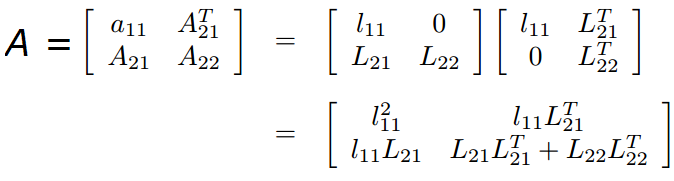
\includegraphics{img/chol.png}

Siendo $a_{11}$ el elemento de la posición (1,1) de A, $A_{21}$ una matriz de (n-1)*1, y $A_{22}$ una matriz de (n-1)*(n-1). Por lo tanto podemos desarrollar el siguiente algoritmo recursivo:

\begin{codesnippet}

    $Cholesky(A^{n*n})$:\\
    \tab $l_{11} =  \sqrt[2]{a_{11}}$ \\
    \tab $si$ $n > 1$ \\
    \tab \tab $L_{21} =  A_{21}/l_{11}$ \\
    \tab \tab $L_{22} =  Cholesky(A_{22}-L_{21}$*$L_{21}^{T})$ \\
\end{codesnippet}

Como se efectúan n llamados recursivos, y en cada uno se hace una resta de matrices, la complejidad asintótica total del algoritmo es $O(n^3)$. A la hora de implementarlo eliminamos la recursión, reemplazandola por un approach iterativo, que es más eficiente. Por lo tanto el algoritmo final quedó así:

\begin{codesnippet}
    $Cholesky(A^{n*n})$:\\
    \tab Para i de 1 hasta n: \\
    \tab \tab $A_{ii} = \sqrt[2]{A_{ii}}$ \\
    \tab \tab Para j de i+1 hasta n: \\
    \tab \tab \tab $A_{ij} = A_{ij}/A_{ii}$ \\
    \tab \tab Para j de i+1 hasta n: \\
    \tab \tab \tab Para k de i+1 hasta j: \\
    \tab \tab \tab \tab $A_{jk} = A_{ji}*A_{ki}$ \\
\end{codesnippet}

En la implementación, el codigo solo necesita la parte triangular inferior de la matriz para funcionar, utilizando asi, la mitad de espacio. Por último cabe destacar que si bien la factorización de Cholesky hace menos operaciones que la de Gauss, n operaciones son raices cuadradas, que computacionalmente son mucho mas caras que sumas y restas. Por lo tanto implementamos una funcion en assembler que calcula la operación sqrt(double) por hardware. Si bien la ganancia en performance no es tanta (aprox 3$\%$), decidimos dejarla porque nos pareció un factor que esta bueno tenerlo controlado para los benchmarks.

\begin{codesnippet}
\end{codesnippet}

\subsection{Benchmarks}

\subsubsection{Performance y complejidades}

 En esta sección evaluaremos los algoritmos en el peor caso, esto es, en matrices con pocos ceros. Los "fixtures" que le dan valores a la matriz de Colley fueron generados al azar, pero siempre controlando que el $\%$ de ceros no baje del $\%$90.
 Primero veamos un grafico que compara la performance de los 3 algoritmos desarrollados:
 
 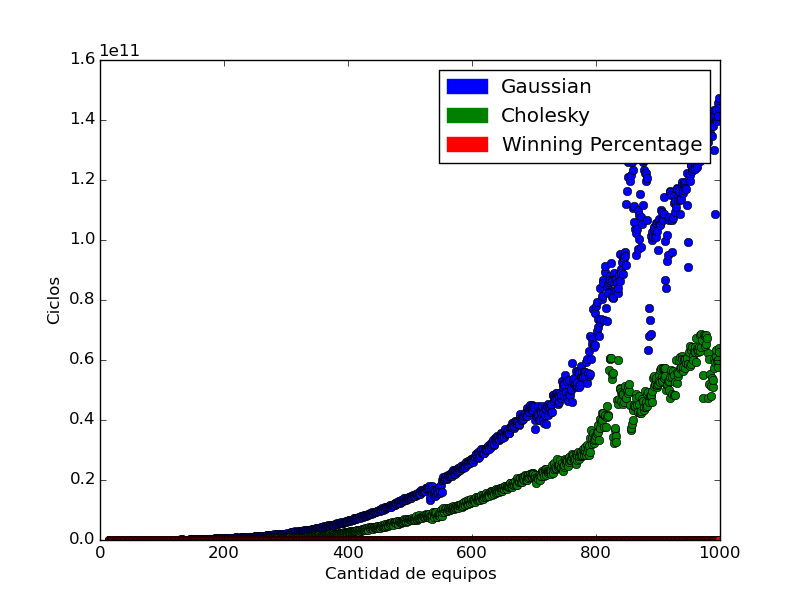
\includegraphics[scale=0.8]{img/testciclos.png}
 
 Como era de esperarse, winning percentage es notablemente mas rápido (tanto que aparece pegado al eje x), ya que tiene una complejidad lineal, mientras que los otros cubica. Lo segundo que vamos a apreciar es que a partir de 700 equipos las mediciones se vuelven bastante mas inestables. Esto se debe a 2 factores: El mas importante es que como utilizamos hash_maps y generamos tests al azar, es de esperarse que el tiempo de acceso a un valor del diccionario no sea completamente uniforme en todos los casos. Por otro lado, nosotros calculamos los tiempos de cómputo directamente del procesador, por lo tanto, como cada medición es extremadamente precisa, es normal que haya varianza entre mediciones. Cabe destacar además, que para n$<$500 también hay variaciones de aprox $\%10$, pero no se aprecian por la escala del gráfico.
 Por último podemos ver que cholesky tarda menos en computarse que gaussian elimination, pero cuánto más?, veamos en el siguiente grafico que divide la cantidad de ciclos de Gaussian por la de Cholesky:
 
 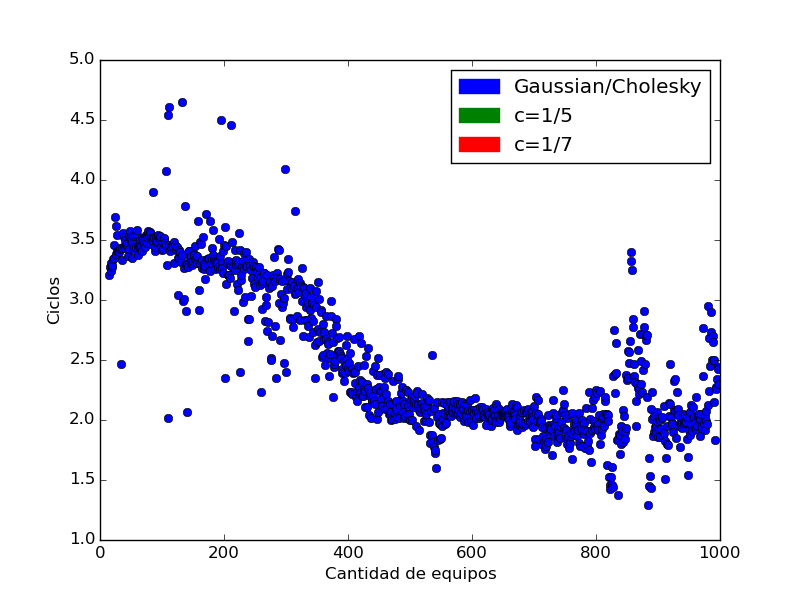
\includegraphics[scale=0.7]{img/gaussianvscholesky.png}
 
 Increiblemente, para sistemas densos con pocos equipos Cholesky es hasta 3.5 veces mas rápido. Hasta aprox 350 equipos se mantiene 3 veces más rápido, luego la diferencia se achica rápidamente, y ya para 420 equipos en adelante se estabiliza en el doble de rápido. Por la inestabilidad debatida antes, el gráfico presenta "anchura". Cabe destacar, que aunque haya habido algunos outliers, nunca en las mil corridas realizadas Cholesky fue más lento que Gaussian.
 
 Veamos ahora si los algoritmos se comportan de acuerdo a su complejidad asintótica. El primer gráfico de la página siguiente muestra la performance de Gaussian Elimination, dividida por $n^2$, $n^3$ y $n^4$. Esto nos da una idea de su crecimiento asintótico para situaciones con hasta 1000 equipos. Esta cota nos pareció mas que suficiente para analizar el comportamiento que tendría en situaciones reales.
 
 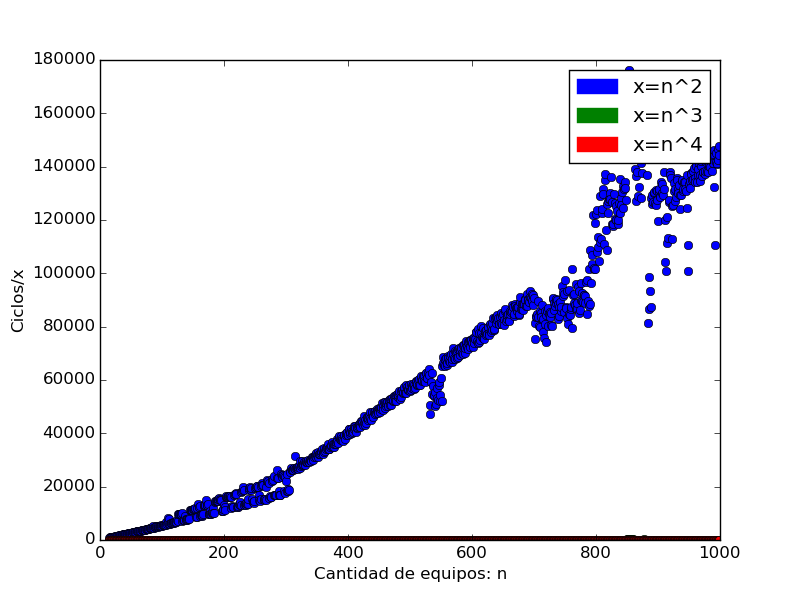
\includegraphics[scale=0.7]{img/complejidadgaussian.png}
 
 Al ver que dividiendo por $n^2$ diverge claramente, y que dividiendo por $n^4$ y $n^3$ la curva queda completamente pegada al eje x, podemos concluir que la complejidad debería ser $O(n^3)$. En el siguiente gráfico probamos dividiendo por $n^3$ con diferentes constantes.
 
  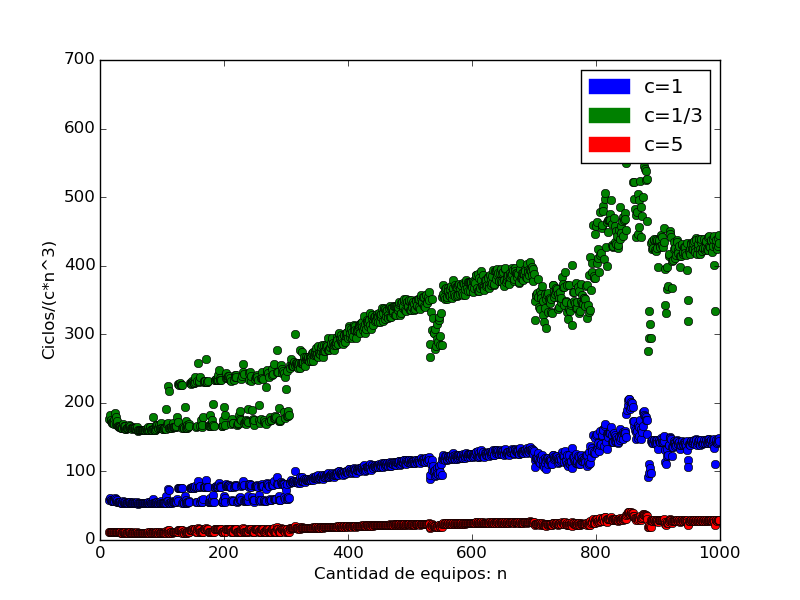
\includegraphics[scale=0.7]{img/constantegaussian.png}
 
 Si bien por el gráfico anterior pensamos que las constantes iban a ser menores a 1, podemos ver que incluso con c$=$1 la curva crece lentamente. Sin embargo, para c=5 la curva que practicamente estable.
 Por lo tanto podemos concluir que el algoritmo para n $\leq$ 1000 tiene un crecimiento asintótico de $O(n^3)$ con una constante un poquito mayor a 5.

 Veamos ahora la complejidad de Cholesky para matrices densas:
 
  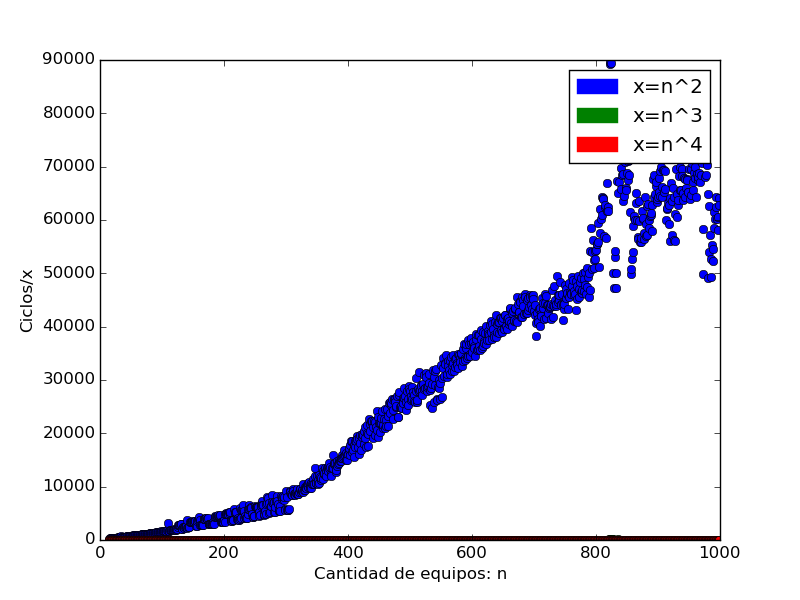
\includegraphics[scale=0.7]{img/complejidadcholesky.png}
  
 Observamos el mismo panorama que para Gauss, vayamos al analisis de constante:
 
  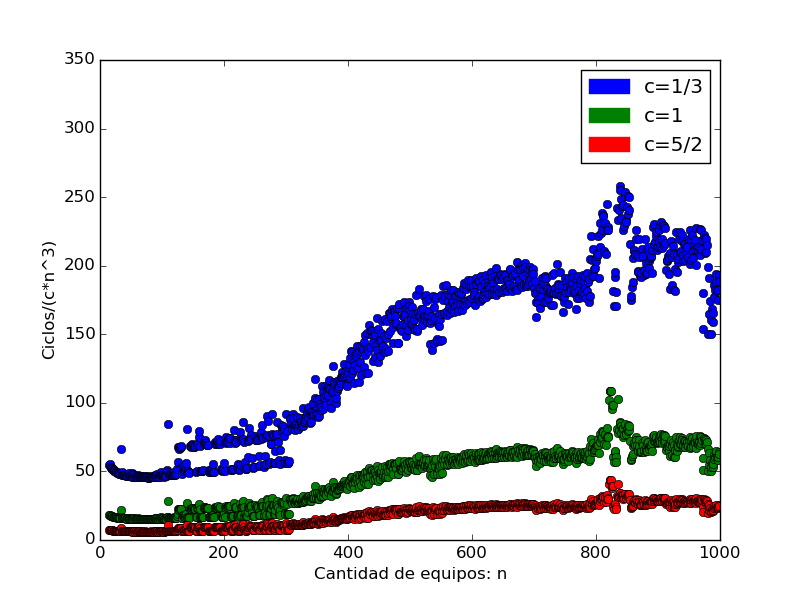
\includegraphics[scale=0.7]{img/constantecholesky.png}
  
 Antes vimos que cholesky es aproximadamente el doble de rápido, gracias a dios la lógica entre experimentos se mantiene, y obtenemos que la constante del algoritmo es un poquitito mas de 2.5, es decir, la mitad que la constante de Gaussian Elimination.
 
 Por último veamos la performance de los algoritmos, dada una cierta cantidad de equipos fija, pero variando la cantidad de ceros en la matriz. En el siguiente gráfico se muestra la cantidad de ciclos consumida por ambos algoritmos con n fijado en 700 y variando la densidad de la matriz:
 
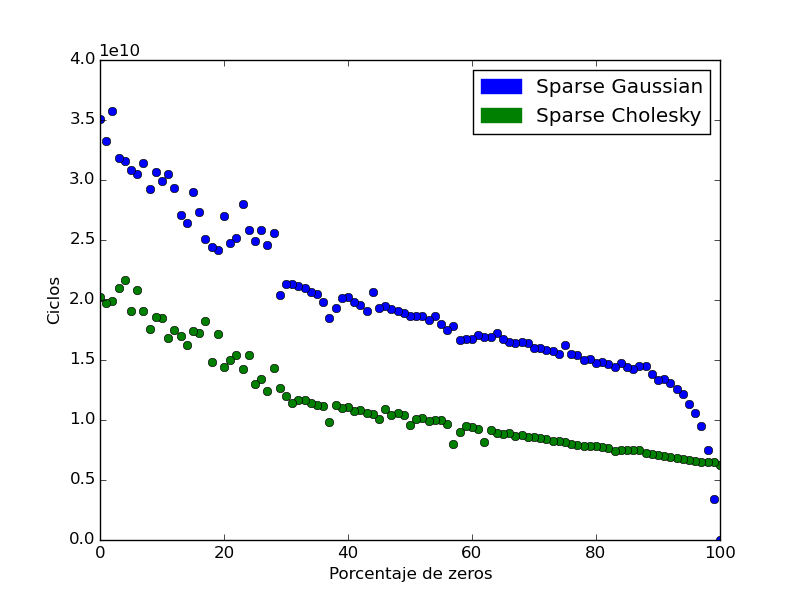
\includegraphics[scale=0.7]{img/testsparse.png}
 
Claramente se ve que hay una diferencia de performance para distintos niveles de densidad de la matriz, sobretodo para Gaussian Elimination. También podemos notar que la brecha de velocidad entre ambos algoritmos se va achicando a medida que la matriz es mas esparsa, e incluso termina con Cholesky siendo mas lento. Por todo todo esto decidimos hacer la siguiente sección 
 
\subsubsection{Matrices esparsas}

Pasemos ahora a ver el comportamiento en matrices esparsas. Primero veamos la diferencia de performance entre Gaussian Elimination y Cholesky con 700 equipos y variando el porcentaje de ceros.

 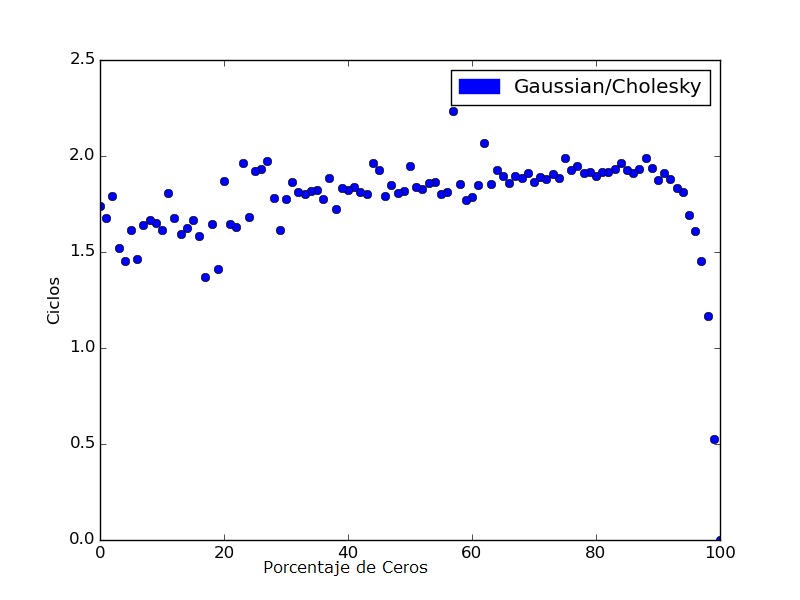
\includegraphics[scale=0.7]{img/sparsegaussianvscholesky.png}
 
 Como venimos viendo, Gauss se beneficia más por la presencia de muchos ceros en la matriz, en este caso vemos que en matrices esparsas por lo general Cholesky sigue siendo mas rápido, pero ahora entre 1.5 y 2 veces mas rápido. También podemos observar que para matrices muy muy esparsas, o sea con 98$\%$ ceros o más, Gaussian Elimination pasa a ser más rápido que Cholesky. Como ya mencionamos antes, la notable mejora es porque las restas entre filas se hacen iterando solo sobre números distintos a cero.
 
 Ahora vamos a ver si las complejidades asintóticas cambian. Primero pensamos en dejar una cantidad de números distinta a cero fija y variar la cantidad de equipos. El problema con este experimento es que después de cierto punto significaría agregar equipos que juegan 0 partidos, y este escenario es demasiado irreal. Por lo tanto optamos por dejar fijo el $\%$ de ceros de la matriz e ir subiendo la cantidad de equipos. En el siguiente gráfico se muestra la performance de los algoritmos en matrices con 90$\%$ ceros:
 
 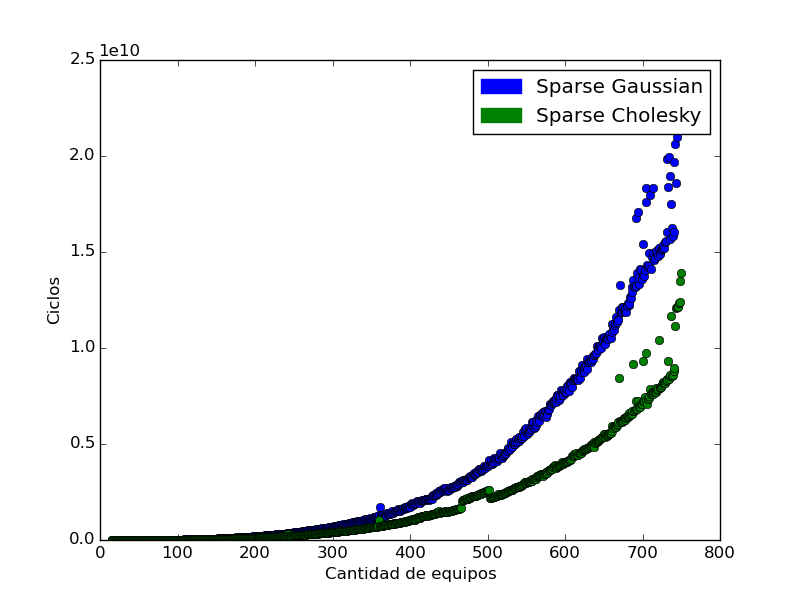
\includegraphics[scale=0.7]{img/testfixedsparse.png}

 Lo primero que no puede ver es que los algoritmos son muchisimo mas estables, es decir, que no hay mucha varianza en los tiempo de medición. Esto tiene sentido, ya que muchos ceros en la matriz implica pocos elementos en los hash_maps, y por lo tanto tiempos de acceso constantes. Lo segundo que vamos a remarcar es que bajó un orden de magnitud con respecto a la performance de matrices densas, es decir, los algoritmos llegan a ser hasta 10 veces mas rápidos en matrices esparsas. Veamos como queda la complejidad asintótica de cada uno, la primer imagen corresponde a Gaussian elimination y la segunda a Cholesky:
 
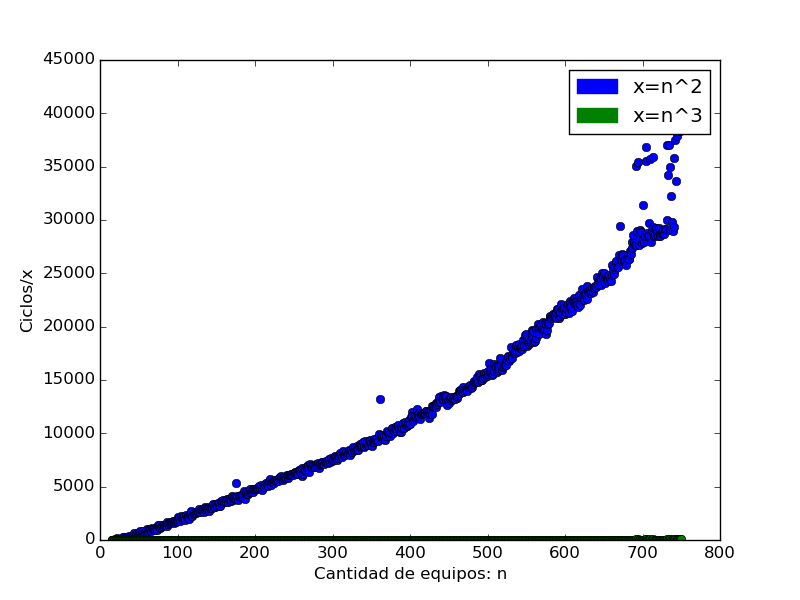
\includegraphics[scale=0.7]{img/complejidadfixedgaussian.png}
  
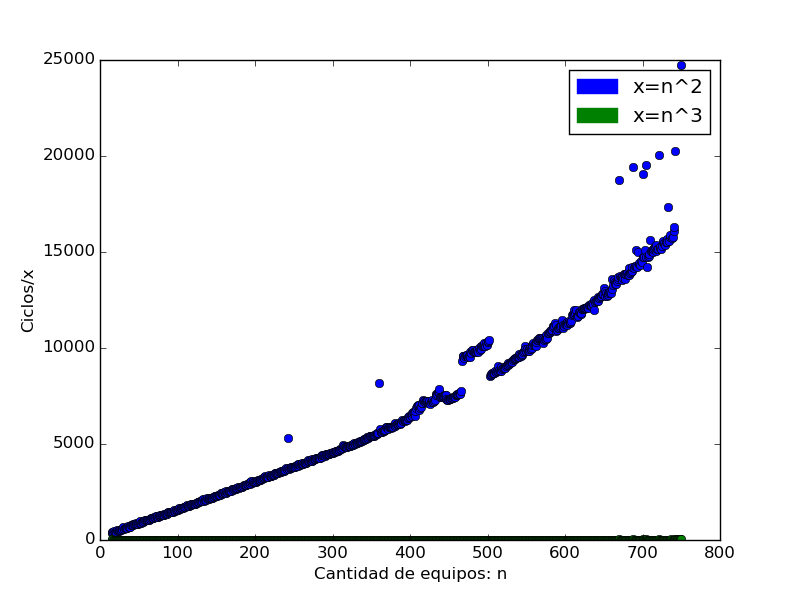
\includegraphics[scale=0.7]{img/complejidadfixedcholesky.png}

Lamentablemente incluso teniendo 90$\%$ de ceros, los algoritmos siguen siendo cúbicos. Sin embargo como vamos a ver en los siguientes gráficos, primero para Gaussian y luego con Cholesky, las constantes sí son mejores.

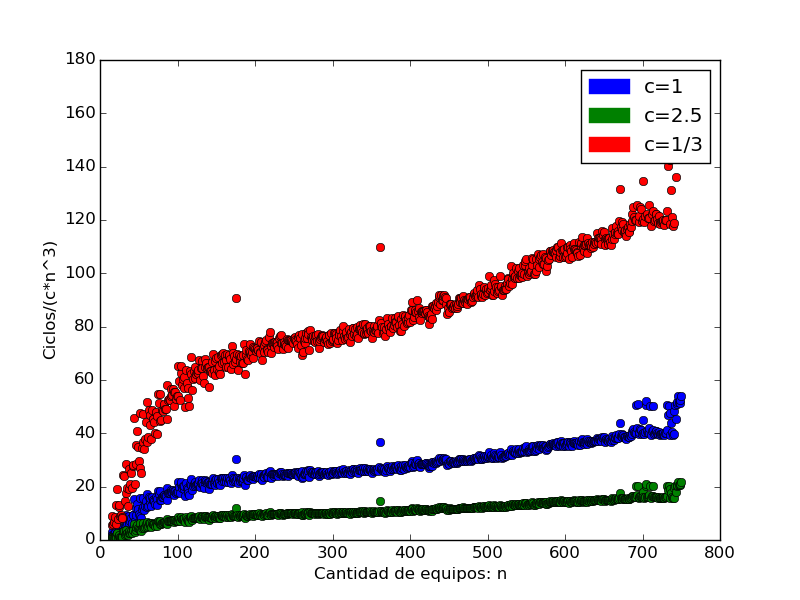
\includegraphics[scale=0.7]{img/constantefixedgaussian.png}
  
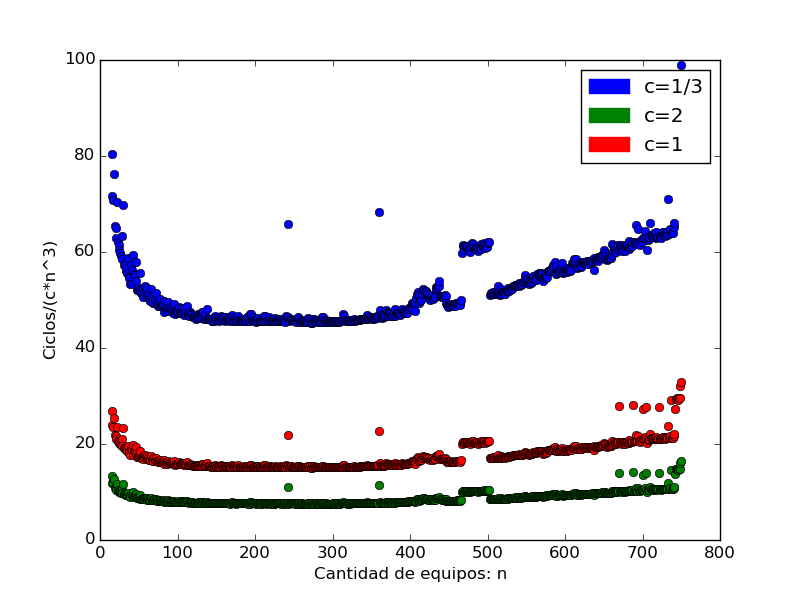
\includegraphics[scale=0.7]{img/constantefixedcholesky.png}

Para matrices densas las constantes eran 5 para Gaussian y 2.5 para cholesky, en este caso bajaron a 2.5 y 2.

Por lo tanto podemos concluir que la estructura planteada es una muy buena elección para matrices esparsas, ya que ademas de poder ahorrar mucho espacio tiene una buena performance, logrando resolver sistemas de 1000 equipos en segundos. Por otro lado, para casos densos no es una buena idea, ya que la cantidad de espacio consumida es la misma y los tiempos de acceso a los hash_maps se vuelven lentos. Es por esto que convendría hacer una heurística analizando datos estadísticos que en base a la cantidad de equipos del sistema a resolver, y al nivel de densidad de la matriz, decida si utilizar un simple array bi-dimensional o la estructura analizada en esta sección.

